\question 有一个矩阵为100行×200列,即a{[}100{]}{[}200{]}。在一个虚拟系统中,采用LRU算法。系统分给该进程5个页面来存储数据(不包含程序),设每页可存放200个整数,该程序要对整个数组初始化,数组存储时是按行存放的。试计算下列两个程序各自的缺页次数(假定所有页都以请求方式调入)(
)。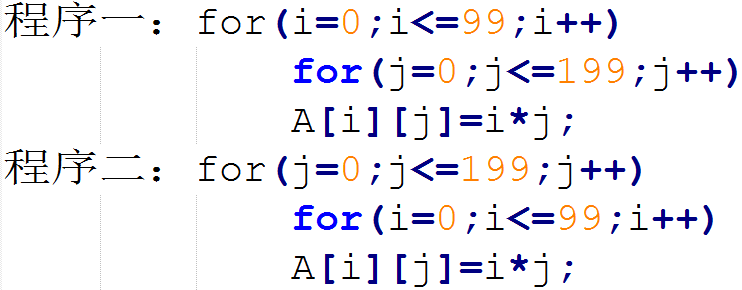
\includegraphics[width=2.42708in,height=0.94792in]{computerassets/E52E0CBF83A575BF60173AB625D4B4A7.png}
\par\twoch{100,200}{\textcolor{red}{100,20000}}{200,100}{20000,100}
\begin{solution}本题中,矩阵a有100×200=20000个整数,每页存放200个整数,故一页可以存放一行数组元素。系统分配给进程5个页面存放数据,假设程序已调入内存(因题目中没有提供与程序相关的数据,故可以不考虑程序的调入问题),因此只需考虑矩阵访问时产生的缺页中断次数。
对于程序一,由于矩阵存放是按行存储,本程序对矩阵a的访问也是按行进行的。因此本程序依次将矩阵a的内容调入内存,每一页只调入一次,每一页都会发生一次缺页中断,因此会产生20000/200=100次缺页中断。
对于程序二,矩阵存放时按行存储,而本程序对矩阵a的访问是按列进行的。当j=0时,内层循环的执行将访问第一列的所有元素,需要依次将矩阵a的100行调入内存,将产生100次缺页中断。当j=1时,仍需要依次将矩阵a的100行调入内存(因留在内存中的是第95、96、97、98、99行),仍将产生100次缺页中断。后续循环,可依次类推。由此可知,程序二将产生20000次缺页中断。
\end{solution}
\question 下面算法中不属于页式虚拟存储管理中的页面调度算法的是
\par\twoch{先进先出调度算法}{最近最少使用调度算法}{\textcolor{red}{优先数调度算法}}{最近最久未使用调度算法}
\begin{solution}优先数调度算法是处理机调度的算法。
\end{solution}
